\chapter{Classical Magnetism and Magnons}

Last session closed on a sentence worth repeating exactly, because it is the sentence that opens
today's lecture too: the same Hubbard-like Hamiltonian can mean-field into either a superconductor
or a magnet, and magnetism was deferred to the next recording. Today is that next recording. We
already met a first pass at mean-field magnetism all the way back in session 1 (the Hubbard chain,
the magnetization $m$, the Mott gap), but that was deliberately left as an appetizer: a sign flip
away from the superconducting case, worked out just far enough to show that magnetism \emph{is} a
symmetry-broken mean-field state. Today we go much further. We will solve the Hubbard model's
magnetism numerically and see ferromagnetism and antiferromagnetism compete as two genuinely
different self-consistent solutions of the same Hamiltonian; we will find the precise threshold
interaction strength above which magnetism appears at all; and then, because that threshold sits
exactly where mean-field theory itself becomes unreliable, we will leave mean field behind and
derive, from first principles, the effective spin Hamiltonian that governs the strongly correlated
limit: the Heisenberg model. From there we go one level further still and ask about the \emph{excitations}
living on top of a magnetically ordered state, which brings us to magnons, the magnetic analogue of
a phonon, built rigorously via the Holstein-Primakoff transformation. And once we have a genuine
band structure for magnons, we will find that the topological machinery from sessions 3 and 4,
Chern numbers, Berry curvature, chiral edge states, applies to them too, giving us topological
magnon bands as a third application of a tool we have now used on electrons twice and on magnons
once.

One piece of framing before we start, because it explains how this session ends. Today's recording
is a single, self-contained lecture on classical magnetism and magnons only; it does not also carry
a second recording on quantum magnetism and the Kondo model the way it might sound from the opening
preview of spinons below. That material genuinely belongs to its own session later in the course.
What is true, and worth saying plainly rather than papering over, is that today's recording simply
stops once it reaches the end of the ``topological magnons'' material: there is no closing take-home
summary slide narrated at the end, the lecture just runs out of planned material. So these notes end
the same way, on topological magnons, without inventing a wrap-up sentence the lecture itself never
says.

\section{Two classes of magnets, and the excitations that live on each}

Let us start by drawing the map of where we are headed, because today's lecture actually previews
material from two future sessions before settling into its own. There are two big classes of
magnetic system.

The first class is magnets that break time-reversal symmetry. These are materials with a net
magnetization on every site (or a staggered one), and a finite spin angular momentum is precisely
what makes a system look different when its ``movie'' is run backwards, which is the definition of
broken time-reversal symmetry. Ferromagnets, antiferromagnets, and noncollinear spin spirals all
belong here. Iron and cobalt are the two materials the lecture actually names, repeatedly, as
concrete examples of this family. This is the class we spend all of today on.

The second class is magnets that do \emph{not} break time-reversal symmetry, at least not classically:
quantum magnets, among them quantum spin liquids. These have a local moment on every site, but the
spins are in quantum superposition rather than settling into a static classical arrangement, so
time-reversal symmetry need not be broken overall. A related case, also mentioned today only in
passing, is the heavy-fermion Kondo system: a combination of local moments in quantum superposition
together with an itinerant metallic electron sea. (The ``Classical and quantum magnetism'' slide
illustrates all three families with material photographs, iron for the ferromagnet/antiferromagnet
family, herbertsmithite for quantum spin liquids, samarium hexaboride SmB$_6$ for heavy-fermion
insulators, but none of those three compound names is actually spoken in this year's narration; they
are slide-only labels, worth knowing about but not something the lecture itself says out loud.)

Each class comes with its own emergent excitation. Time-reversal-breaking magnets host \textbf{magnons}:
spin-1, charge-neutral fluctuations of the order parameter, the direct magnetic analogue of a
phonon. Because magnons carry no charge, they are completely unaffected by electric fields, and they
can propagate in materials that are electronic insulators: a ferromagnetic (or antiferromagnetic)
Mott insulator lets no current through, yet a magnon can still carry spin and heat across it.
Quantum magnets instead host \textbf{spinons}: spin-$1/2$, charge-neutral excitations, sometimes
described informally as ``half an electron,'' since an electron's spin and charge degrees of freedom
have effectively separated. We will build magnons carefully over the rest of today's session.
Spinons, and the Kondo lattice model, are only previewed here as a name and a spin quantum number;
their full construction is a later session's material (session 8), not something today's lecture
returns to.

\section{A recap: symmetry breaking and the mean-field philosophy}

We have seen this move twice already in this course, first in session 1 in miniature, then in full
depth for superconductivity in session 5, so let us state it once more, briskly, before putting it
to work on magnetism specifically. Many-body interactions can spontaneously break a symmetry that
the Hamiltonian itself possesses. Three cases run through this entire course: magnets break
time-reversal (equivalently, real-space spin-rotation) symmetry; charge density waves break lattice
translational symmetry; superconductors break gauge symmetry. All three emerge from the same generic
starting point, a kinetic (single-particle, exactly solvable) term plus a quartic many-body
interaction, and all three are extracted the same way: mean-field theory factorizes the quartic term
by replacing part of it with its expectation value, turning an intractable many-body problem into a
solvable single-particle one, solved self-consistently.

Where do the interactions themselves come from? Two sources. Electrostatic (Coulomb) repulsion
between electrons is the classical, always-present contribution. Interactions can also be mediated
by other quasiparticles (phonons, magnons, plasmons), which can flip the \emph{net} effective interaction
from repulsive to attractive. Magnetism specifically needs the net interaction to be repulsive; since
bare Coulomb repulsion is already repulsive, this is the easy case to realize, which is one reason
magnetism is so common in nature.

\section{The Hubbard model and mean-field magnetism, revisited}

The minimal Hamiltonian for all of this is the one-dimensional Hubbard chain we first met in
session 1,

\begin{equation}
H = -t\sum_{n,\sigma}\left(c_{n\sigma}^\dagger c_{n+1,\sigma} + \text{h.c.}\right) + U\sum_n c_{n\uparrow}^\dagger c_{n\uparrow}\, c_{n\downarrow}^\dagger c_{n\downarrow},
\end{equation}

hopping $t$ plus a purely local (on-site) density-density interaction between opposite spins, the
Hubbard term. Negative $U$ (attractive) drives superconductivity, session 5's territory; positive $U$
(repulsive) drives magnetism, ours today.

The mean-field decoupling proceeds exactly as before: replace $c_{n\uparrow}^\dagger c_{n\uparrow}$
and $c_{n\downarrow}^\dagger c_{n\downarrow}$ by their expectation values, leaving a bilinear
Hamiltonian with spin-dependent on-site energies. Nothing forces these two expectation values to
agree, and the imbalance between them is exactly the magnetization,

\begin{equation}
m = \langle c_\uparrow^\dagger c_\uparrow\rangle - \langle c_\downarrow^\dagger c_\downarrow\rangle,
\end{equation}

which plays the role of an exchange field: the resulting mean-field Hamiltonian looks schematically
like $H_\text{MF} \sim -\tfrac{U}{2}\, m\, \boldsymbol\sigma\cdot c$, where $\boldsymbol\sigma$ is the
vector of Pauli matrices. Self-consistency gives $m=0$ for $U<0$ and a genuinely magnetic $m\neq 0$
for $U>0$, exactly as in session 1.

Here is a piece of rigor the slides show but the spoken explanation only gestures at: nothing in this
construction singles out the $z$ axis. The Hubbard interaction can be rewritten exactly, for a single
site, in terms of the local spin operator $\mathbf{S} = \tfrac12 c_\alpha^\dagger \boldsymbol\sigma_{\alpha\beta} c_\beta$
and the total occupation $n = n_\uparrow + n_\downarrow$, as
$U\, n_\uparrow n_\downarrow = \tfrac{U}{4}n^2 - U\mathbf{S}^2$ (up to the usual $n^2=n+2n_\uparrow n_\downarrow$
identity for fermionic occupation numbers). Mean-field theory then factorizes the quadratic operator
$\mathbf{S}^2$ the same way it factorizes any product of two operators, $\mathbf{S}^2 \approx
2\langle\mathbf{S}\rangle\cdot\mathbf{S} - \langle\mathbf{S}\rangle^2$, and the resulting exchange
field points along $\mathbf{m} \equiv \langle\mathbf{S}\rangle$, in \emph{whichever} direction that
expectation value happens to be nonzero. Choosing $\langle c_\uparrow^\dagger c_\uparrow\rangle \neq
\langle c_\downarrow^\dagger c_\downarrow\rangle$, as in (6.2), picks out $m_z\neq 0$; choosing instead
$\langle c_\uparrow^\dagger c_\downarrow\rangle \neq 0$ picks out $m_x$ or $m_y$. Mean-field magnetism
is therefore not restricted to the $z$ axis at all: it produces magnets with magnetization along any
direction in space, including genuinely noncollinear arrangements where $\mathbf{m}$ points in
different directions on different sites. This is exactly the ``non-collinear mean-field Hamiltonian''
figure on the slides, which the spoken lecture only names in passing.

Mean field is only trustworthy when $U \ll t$; we will see in Section 6.6 that magnetism typically
needs the opposite regime, which is precisely why the strongly localized limit of Section 6.7 onward
matters so much.

\section{Numerical mean-field magnetism: exchange splitting and antiferromagnetic order}

Let us see the machinery of Section 6.3 actually run. First take the one-dimensional chain (6.1)
with a single-site unit cell at 20\% filling and solve it self-consistently. The resulting band
structure exchange-splits: the spin-up band (occupied up to the chemical potential) sits at lower
energy than the spin-down band (empty at this filling), and the splitting between them, the
\textbf{exchange splitting}, grows with $U$. Since only spin-up states are occupied, this is a fully
polarized ferromagnetic solution with $m\neq 0$.

Now enlarge the unit cell to two sites and work at half filling instead. At $U=0$ there are two
bands (one per site in the cell), crossing at one point: the system is metallic. Turning on $U>0$
opens a mean-field gap, and in real space the two sublattices develop opposite spin polarization: one
site mostly up, its neighbor mostly down. The \emph{net} magnetization is zero, but the \emph{staggered}
magnetization is not: this is antiferromagnetic order, and (as always with mean-field gap opening)
it lowers the total electronic energy relative to the ungapped state, because the states that get
pushed down in energy by the gap are exactly the occupied ones.

\begin{notebookbox}{\texttt{session6.ipynb}, ``(Reminder) Bandstructure of a tight binding chain with two sites'' and ``(Exercise) Magnetic order driven by interactions in a chain''}
Start from the two-site, non-interacting band structure (the metallic crossing case), then switch
on $U$ and watch the mean-field gap open and the real-space spin pattern become antiferromagnetic,
reproducing (6.2)'s exchange splitting directly. The single-site, 20\% filling ferromagnetic case
from the same section is the companion calculation.
\end{notebookbox}

\section{Ferromagnet versus antiferromagnet: which one wins?}

The Hubbard chain (6.1) admits \emph{both} a ferromagnetic self-consistent solution (single-site cell,
metallic, gapless) and an antiferromagnetic one (two-site cell, insulating, gapped) at the same
filling and the same $U$. Both are genuine fixed points of the self-consistency loop; only one can be
the true ground state, and we settle that by comparing total energies. The gapped antiferromagnetic
solution always wins here: opening a gap pushes the occupied single-particle energies down, so the
insulating configuration has lower total energy than the gapless ferromagnetic one at every $U>0$ we
can reach numerically in this half-filled chain.

It is worth tracking how large that energy advantage is as a function of $U$. At $U=0$ the two
configurations are identical, so the energy difference vanishes. As $U$ grows from zero the gap opens
and the energy difference grows with it. But then, surprisingly, as $U$ keeps growing the energy
difference starts \emph{shrinking} again, and in the $U\to\infty$ limit (equivalently, the limit where the
kinetic energy becomes negligible) the two configurations become degenerate. Numerically this energy
difference fits a $1/U$ functional form. We are going to rederive this exact $1/U$ scaling
analytically in Section 6.8, from a completely independent calculation, as a genuine cross-check
between the mean-field numerics and a many-body perturbative treatment.

\section{A criterion for magnetism: the Stoner threshold}

A natural question: does \emph{any} repulsive $U>0$ produce magnetism, or is there a threshold? Write the
mean-field bands as $E_\sigma(\mathbf{k}) = E(\mathbf{k}) - \sigma\, \tfrac{U}{2}m$ for
$\sigma=\pm1$ (spin up/down), with $m$ the self-consistent magnetization of (6.2). At zero
temperature, self-consistency reads

\begin{equation*}
m = \sum_{\mathbf k}\Big[n_F\big(E(\mathbf k)-\tfrac{U}{2}m\big) - n_F\big(E(\mathbf k)+\tfrac{U}{2}m\big)\Big].
\end{equation*}

Expanding the right-hand side for small $m$ gives $m \approx U\,m\,D(E_F)$, where $D(E_F)$ is the
density of states at the Fermi level. This has the trivial solution $m=0$ always, but a \emph{nontrivial}
solution branches off exactly when the linear coefficient reaches one:

\begin{equation}
U\, D(E_F) \geq 1.
\end{equation}

This is the Stoner criterion. Below threshold only $m=0$ is stable, and the system is nonmagnetic no
matter how you perturb it; above threshold the nonmagnetic solution becomes unstable and a finite $m$
develops spontaneously. This is exactly why some metals with sizable Coulomb repulsion, aluminum or
lead, stay nonmagnetic: their density of states at the Fermi level is too small for the product in
(6.3) to clear one. Iron and cobalt, by contrast, combine a large density of states (from narrow $d$
bands) with a sizable effective $U$, comfortably clearing the threshold. Numerically, this shows up
exactly as (6.3) predicts: the self-consistent magnetization of the chain stays pinned at zero below
a critical $U$, then grows continuously once $U$ crosses that threshold. Figure~\ref{fig:s06:stoner}
shows both halves of this statement at once: why a nontrivial solution of the self-consistency
condition only exists above threshold, and what the resulting magnetization curve looks like.

% Session 6 -- the Stoner criterion.
% Placement: sec. "A criterion for magnetism: the Stoner threshold", right after eq. (6.3).
% Rendered by figures/blender/s06f01_stoner.py, labels in figures/overlays/s06f01_stoner.tex.
\begin{aqmfigure}{fig:s06:stoner}{A graphical reading of the Stoner criterion (6.3). (a) The
self-consistency condition $m=f(m)$, where $f$ is the right-hand side of the zero-temperature gap
equation, drawn here with the shape $\tanh$ for two values of the slope. It is an odd function that
saturates once the bands are fully polarized, and its slope at the origin is exactly $U D(E_F)$. If
this slope is below one, the only crossing with $y=m$ is the trivial solution $m=0$. Once the slope
is above one, a pair of nontrivial solutions $\pm m_0$ appears and the nonmagnetic state becomes
unstable. (b) The resulting order parameter, which stays at zero until $U D(E_F)$ reaches one and
then grows continuously. For this reason, whether a metal becomes magnetic is not decided by $U$
alone but by the \emph{product} of $U$ with the density of states at the Fermi level. This is why
aluminium and lead stay nonmagnetic even with a sizeable Coulomb repulsion, while the narrow $d$
bands of iron and cobalt are clearly above the threshold.}
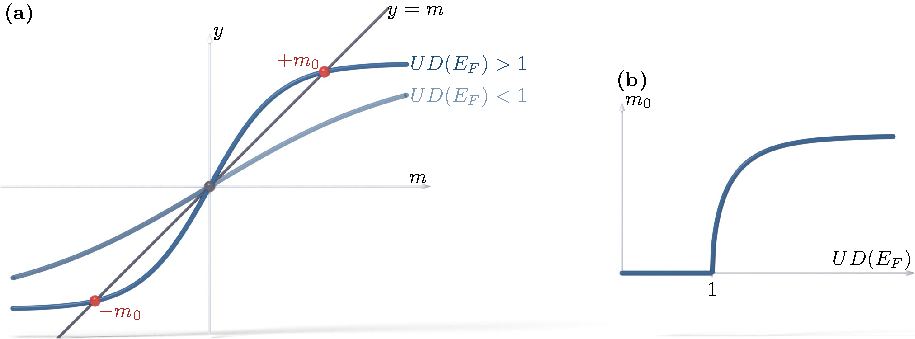
\includegraphics{figures/pdf/s06f01_stoner.pdf}
\end{aqmfigure}


\begin{notebookbox}{\texttt{session6.ipynb}, ``(Exercise) Intermediate coupling regime and Stoner instability''}
Reproduce the threshold behavior of (6.3) directly: scan the self-consistent magnetization as a
function of $U$ and locate the critical interaction where $m$ first becomes nonzero.
\end{notebookbox}

\begin{notebookbox}{\texttt{session6.ipynb}, ``(Exercise) Magnetism in flat bands''}
A flat band has (in principle) a divergent density of states at $E_F$, so the Stoner product
$U D(E_F)$ in (6.3) clears threshold for essentially any $U>0$. This exercise is not narrated in
the transcript, but it is the natural numerical extension of Section 6.6: a flat-band system is
the ``easiest possible'' case for magnetism to appear.
\end{notebookbox}

One important consequence closes this section and opens the next: (6.3) tells us that magnetism
generically wants $U D(E_F) \gtrsim 1$, and for a reasonable bandwidth that typically means $U$ needs
to be comparable to or larger than $t$, not smaller. But mean-field theory itself is only reliable for
$U \ll t$ (Section 6.3). So the regime where magnetism actually shows up is, generically, exactly the
regime where the tool we have been using breaks down. We need a genuinely different approach for
$U \gg t$, and that is what the rest of this session builds.

\section{Where mean field breaks down: the strongly localized limit}

Let us look again at the half-filled chain from Section 6.4, but now track the magnetization per site
as $U$ grows from zero to very large values. At $U=0$ there is no interaction and $m=0$. As $U$
increases, $m$ grows, and as $U\to\infty$ it saturates at exactly one Bohr magneton per site: a full,
localized spin-$1/2$ moment on every site, pointing in alternating directions from one sublattice to
the next (the ``Ising-like'' antiferromagnetic state the numerics converge to).

This saturation is telling us something physical: in the large-$U$ limit electrons stop moving
altogether. Hopping an electron onto an already-occupied neighboring site costs an energy $U$, and
once $U\gg t$ that cost is prohibitive, so each site simply keeps its one electron, localized, with
only its spin free to fluctuate. The right way to organize perturbation theory in this limit is
therefore \emph{not} around the kinetic term (as mean field implicitly does), but around localization
itself: treat the interacting, localized configuration as the zeroth-order ground state, and treat
hopping as a small perturbation on top of it.

\section{From the Hubbard dimer to the Heisenberg model}

Let us make this precise on the smallest possible example: two sites, $0$ and $1$, hopping $t$
between them, local repulsion $U$ on each, and exactly two electrons total (half filling). The Fock
space at this filling has $\binom{4}{2}=6$ states: four with one electron on each site (each site's
electron can independently be up or down) and two with both electrons on the same site (one electron
up, one down, by Pauli exclusion).

Group these by energy in the atomic limit ($t=0$). The four singly-occupied configurations,
$|\!\uparrow,\uparrow\rangle$, $|\!\downarrow,\downarrow\rangle$, $|\!\uparrow,\downarrow\rangle$,
$|\!\downarrow,\uparrow\rangle$, cost no interaction energy at all: call this the \textbf{low-energy
manifold}, at energy $0$. The two doubly-occupied configurations,
$|\!\uparrow\downarrow,0\rangle$ and $|0,\uparrow\downarrow\rangle$, each pay the full charging
energy $U$: the \textbf{high-energy manifold}. In the low-energy manifold, every state has exactly one
electron per site, so the charge degree of freedom is completely frozen; only the spin on each site
can still fluctuate. The natural low-energy effective Hamiltonian is therefore a Hamiltonian for spin
alone, and rotational invariance fixes its form up to an overall coupling: $H_\text{eff} = J\,
\mathbf S_0\cdot\mathbf S_1$, the two-site Heisenberg Hamiltonian. What remains is to extract $J$ from
the microscopic $t$ and $U$.

Hopping (the perturbation) conserves total spin, so it cannot connect the low-energy manifold to the
high-energy one for the \emph{parallel}-spin states at all: applying $H_t$ to $|\!\uparrow,\uparrow\rangle$
would require moving a spin-up electron onto a site that already holds one, which Pauli exclusion
forbids outright. The three parallel/triplet-like states ($|\!\uparrow,\uparrow\rangle$,
$|\!\downarrow,\downarrow\rangle$, and the symmetric combination $\tfrac{1}{\sqrt2}(|\!\uparrow,\downarrow\rangle+|\!\downarrow,\uparrow\rangle)$)
are therefore exact eigenstates of the \emph{full} Hamiltonian at energy exactly $E_T=0$: hopping simply
cannot touch them, to any order. The antiparallel/singlet combination
$|S\rangle=\tfrac{1}{\sqrt2}(|\!\uparrow,\downarrow\rangle-|\!\downarrow,\uparrow\rangle)$ is
different: hopping \emph{can} connect it to the (symmetric) doubly-occupied combination
$|D\rangle=\tfrac{1}{\sqrt2}(|\!\uparrow\downarrow,0\rangle+|0,\uparrow\downarrow\rangle)$, with
matrix element $\langle D|H_t|S\rangle = -2t$. Restricted to the two-dimensional subspace
$\{|S\rangle,|D\rangle\}$, the Hamiltonian is exactly

\begin{equation*}
H = \begin{pmatrix} 0 & -2t \\ -2t & U\end{pmatrix},
\end{equation*}

with exact eigenvalues $E_\pm = \tfrac{U}{2}\pm\sqrt{(U/2)^2+4t^2}$. The singlet ground-state energy
is the lower root, $E_S = \tfrac{U}{2}-\sqrt{(U/2)^2+4t^2}$; expanding for $U\gg t$,

\begin{equation*}
E_S \;\approx\; -\frac{4t^2}{U} + O(t^4/U^3), \qquad E_T = 0 \text{ exactly.}
\end{equation*}

Comparing this to the Heisenberg dimer's exact spectrum, $E_\text{singlet}=-\tfrac34 J$ and
$E_\text{triplet}=+\tfrac14 J$ (so the singlet-triplet gap is $\Delta E = E_T-E_S = J$), we read off

\begin{equation}
J = \frac{4t^2}{U}.
\end{equation}

$J>0$: antiferromagnetic, the singlet sits below the triplet. This confirms, with the correct
numerical prefactor, the second-order perturbation theory sketched in the lecture (pristine
Hamiltonian = the Hubbard term, perturbation = hopping, matrix element $t$, energy denominator $U$),
and it reproduces exactly the $1/U$ scaling found numerically for the ferromagnet/antiferromagnet
energy splitting back in Section 6.5: that mean-field energy difference \emph{is} (twice) the exchange
coupling (6.4), so the two completely different calculations, mean-field numerics and many-body
perturbation theory, agree. Figure~\ref{fig:s06:dimer} collects the whole argument: the Pauli
blockade that protects the triplet, the virtual excursion that lowers the singlet, and the exact
spectrum whose splitting is $J$.

% Session 6 -- the Hubbard dimer: why superexchange is antiferromagnetic, and why J = 4t^2/U.
% Placement: sec. "From the Hubbard dimer to the Heisenberg model", after the 2x2 matrix
% and its eigenvalues, at the paragraph that reads off (6.4).
% Rendered by figures/blender/s06f02_dimer.py, labels in figures/overlays/s06f02_dimer.tex.
\begin{aqmfigure}{fig:s06:dimer}{Superexchange in the two-site Hubbard model, and the reason why it
is always antiferromagnetic. (a) With parallel spins, the only possible hop would put two $\uparrow$
electrons on one site, and Pauli exclusion forbids this completely. As a result the triplet states
cannot lower their energy at any order, and stay at exactly $E_T=0$. With antiparallel spins the hop
is allowed, so the singlet goes through a virtual double occupation of energy $U$, the glow, and
comes back, and gains a second-order energy $-4t^2/U$. Here the magnetic order is a purely kinetic
effect, since antiparallel spins have lower energy because only they can move. (b) The exact singlet
energy $E_S=\tfrac{U}{2}-\sqrt{(U/2)^2+4t^2}$ as a function of $U/t$, with $E_T=0$ exact for every
$U$. The singlet-triplet splitting \emph{is} the Heisenberg coupling $J$ of (6.4), and it decays as
$4t^2/U$, the grey curve. This is the same $1/U$ law that we found numerically for the mean-field
energy difference between the ferromagnet and the antiferromagnet in Section 6.5.}
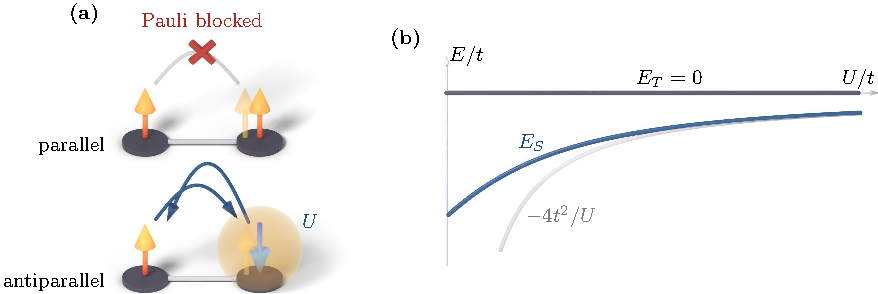
\includegraphics{figures/pdf/s06f02_dimer.pdf}
\end{aqmfigure}


\begin{notebookbox}{\texttt{session6.ipynb}, ``(Reminder) The spectra of a dimer,'' ``(Exercise) The interacting Hubbard dimer,'' ``Gap opening in the Hubbard model,'' and ``(Exercise) The strongly interacting limit''}
Diagonalize the six-state Hubbard dimer directly and confirm the singlet-triplet splitting matches
(6.4). Then push $U/t$ large and check that the gap and the low-energy spectrum converge to the
Heisenberg-model prediction, cross-checking this section's exact result against brute-force
diagonalization.
\end{notebookbox}

\section{The Heisenberg model on a general lattice}

Nothing in Section 6.8's argument used the fact that we had only two sites. For a generic lattice
with hopping $t_{ij}$ between sites $i$ and $j$ and local interaction $U$, the same second-order
argument applies to every bonded pair independently, in the limit $U\gg t_{ij}$, giving the
generalized Heisenberg Hamiltonian

\begin{equation}
H_\text{Heis} = \sum_{\langle ij\rangle} J_{ij}\, \mathbf S_i\cdot\mathbf S_j, \qquad J_{ij} = \frac{4t_{ij}^2}{U}.
\end{equation}

Because $J_{ij}\propto t_{ij}^2$, this superexchange coupling derived directly from a single-orbital
Hubbard model is always positive, antiferromagnetic, regardless of the sign or geometry of $t_{ij}$.
More general (non-Hubbard, multi-orbital) microscopic models can and do produce couplings of either
sign; we will see explicitly in Section 6.11 how ferromagnetic coupling arises once a second,
intermediate orbital gets involved. The sign convention throughout is: $J_{ij}>0$ favors antiparallel
neighboring spins (antiferromagnetic), $J_{ij}<0$ favors parallel neighboring spins (ferromagnetic).
Treating the spins in (6.5) as classical vectors already reproduces both classical ground states on a
two-site bond: antiparallel for $J>0$, parallel for $J<0$.

\section{Bipartite order versus geometric frustration}

On a \textbf{bipartite} lattice, one where the sites split cleanly into two sublattices $A$ and $B$ such
that every bond connects an $A$ site to a $B$ site (square, honeycomb), the antiferromagnetic
Heisenberg model (6.5) has an obvious classical ground state: all spins on $A$ point one way, all
spins on $B$ point the opposite way, satisfying every single bond's preference for antiparallel
neighbors simultaneously. This is exactly the two-sublattice, collinear antiferromagnetic order we
already saw appear at the mean-field level in Section 6.4, and (6.5) explains \emph{why}: in the large-$U$
limit the mean-field Hubbard model on a bipartite lattice literally reduces to this Heisenberg model.

Frustrated lattices are different. On a \textbf{non-bipartite} lattice, kagome or triangular being the
standard examples, there is no way to two-color the sites so that every bond connects opposite
colors; a triangular plaquette, for instance, has three mutually neighboring sites, and no assignment
of up/down spins can make all three bonds antiparallel simultaneously. The antiferromagnetic
tendency of $J_{ij}>0$ is still there on every individual bond, but it cannot be satisfied everywhere
at once: this is \textbf{geometric frustration}. The system's best compromise is typically a noncollinear
arrangement (classic case: spins at $120^\circ$ to each other on a triangular plaquette) that maximizes
the total antiferromagnetic character bond by bond, without fully satisfying any single bond. This
noncollinear character shows up directly in the mean-field solution of the corresponding electronic
Hamiltonian too, not just in the spin-model picture. Figure~\ref{fig:s06:frustration} places the
bipartite case, the frustrated collinear attempt and the $120^\circ$ compromise side by side, with
the classical bond energies that decide between the last two.

% Session 6 -- bipartite order versus geometric frustration.
% Placement: sec. "Bipartite order versus geometric frustration", after the triangular-plaquette
% paragraph that introduces the 120-degree compromise.
%
% Energies are quoted per plaquette for classical spins of length S, so that
% S_i . S_j = S^2 cos(theta_ij): a satisfied (antiparallel) bond contributes -J S^2,
% a parallel bond +J S^2, and a 120-degree bond -J S^2 / 2.
\begin{aqmfigure}{fig:s06:frustration}{How the geometry decides if an antiferromagnet can order.
(a) On a bipartite lattice the sites can be coloured with two colours, every bond joins the two
colours, and the N\'eel state of Section 6.10 satisfies all bonds at the same time. (b) On a triangle
it is not possible to use two colours. If we fix two spins antiparallel, the third one is parallel to
one of its neighbours for any choice, and one bond stays frustrated. For classical spins, this collinear compromise costs $+JS^2$ on the frustrated bond, and the total is
$-JS^2$ per triangle. (c) The energy is lower if no single bond is fully satisfied. Three spins at $120^\circ$ give $\mathbf
S_i\cdot\mathbf S_j=-S^2/2$ on \emph{every} bond and a total of $-\tfrac32 JS^2$, which is lower than
(b) by half of its value. This is the origin of the noncollinear order to which the mean-field
solution of the corresponding electronic Hamiltonian also converges.}

\begin{tikzpicture}[x=1cm, y=1cm]

% --- local helper: a classical spin, dot at (#1,#2), arrow at angle #3 -------
\newcommand{\clspin}[4]{% x, y, angle, colour
  \draw[aqm, draw=#4, -{Stealth[length=4.6pt,width=3.8pt]}]
    ({#1-0.26*cos(#3)},{#2-0.26*sin(#3)}) -- ({#1+0.28*cos(#3)},{#2+0.28*sin(#3)});}

% --- panel headings, all on one baseline ------------------------------------
\node[aqmpanel, anchor=south] at (0.92,2.45) {(a) bipartite};
\node[aqmpanel, anchor=south] at (4.90,2.45) {(b) frustrated};
\node[aqmpanel, anchor=south] at (9.60,2.45) {(c) the $120^\circ$ state};

% ============================ (a) bipartite ==================================
\begin{scope}[shift={(0,0)}]
  \def\dd{0.92}
  \foreach \i in {0,1,2} {
    \draw[aqmbond] (0,\i*\dd) -- (2*\dd,\i*\dd);
    \draw[aqmbond] (\i*\dd,0) -- (\i*\dd,2*\dd);
  }
  % sublattice A: (i+j) even, spins up
  \foreach \i/\j in {0/0,0/2,1/1,2/0,2/2} {
    \node[aqmsite, minimum size=5pt] at (\i*\dd,\j*\dd) {};
    \clspin{\i*\dd}{\j*\dd}{90}{aqmaccent}
  }
  % sublattice B: (i+j) odd, spins down
  \foreach \i/\j in {0/1,1/0,1/2,2/1} {
    \node[aqmsiteopen, minimum size=5pt] at (\i*\dd,\j*\dd) {};
    \clspin{\i*\dd}{\j*\dd}{270}{aqmaccent}
  }
  \node[aqmlabsmall, anchor=north, align=center, text width=4.2cm] at (\dd,-0.55)
    {every bond $\mathbf S_i\cdot\mathbf S_j=-S^2$,\\[1pt]
     \textcolor{aqmaccent}{all satisfied at once}};
\end{scope}

% ============================ (b) frustrated triangle ========================
\begin{scope}[shift={(4.90,0.62)}]
  \def\rr{0.86}
  \coordinate (b1) at (90:\rr);
  \coordinate (b2) at (210:\rr);
  \coordinate (b3) at (330:\rr);
  \draw[aqmbond] (b1) -- (b2);
  \draw[aqmbond] (b2) -- (b3);
  \draw[aqmbondstrong, draw=aqmbroken] (b1) -- (b3);

  \node[aqmsite, minimum size=5pt] at (b1) {};
  \node[aqmsiteopen, minimum size=5pt] at (b2) {};
  \node[aqmsite, minimum size=5pt] at (b3) {};
  \clspin{0}{0.860}{90}{aqmaccent}
  \clspin{-0.745}{-0.430}{270}{aqmaccent}
  \clspin{0.745}{-0.430}{90}{aqmaccent}

  % mark the unsatisfiable bond with a cross at its midpoint
  \draw[aqm, draw=aqmbroken, line width=1.0pt] (0.272,0.115) -- (0.472,0.315);
  \draw[aqm, draw=aqmbroken, line width=1.0pt] (0.272,0.315) -- (0.472,0.115);
  \node[aqmlabsmall, text=aqmbroken, anchor=west] at (0.55,0.30) {$+JS^2$};

  \node[aqmlabsmall, anchor=north, align=center, text width=3.6cm] at (0,-1.17)
    {two bonds $-JS^2$, one bond $+JS^2$,\\[1pt]
     total \textcolor{aqmbroken}{$-JS^2$}};
\end{scope}

% ============================ (c) 120-degree order ===========================
\begin{scope}[shift={(9.60,0.62)}]
  \def\rr{0.86}
  \coordinate (c1) at (90:\rr);
  \coordinate (c2) at (210:\rr);
  \coordinate (c3) at (330:\rr);
  \draw[aqmbond] (c1) -- (c2);
  \draw[aqmbond] (c2) -- (c3);
  \draw[aqmbond] (c1) -- (c3);

  \node[aqmsite, minimum size=5pt] at (c1) {};
  \node[aqmsite, minimum size=5pt] at (c2) {};
  \node[aqmsite, minimum size=5pt] at (c3) {};
  \clspin{0}{0.860}{90}{aqmbroken}
  \clspin{-0.745}{-0.430}{210}{aqmbroken}
  \clspin{0.745}{-0.430}{330}{aqmbroken}

  % the relative angle between two of the three spin directions
  \draw[aqmguide] (0,0) -- (90:0.56);
  \draw[aqmguide] (0,0) -- (330:0.56);
  \draw[aqm, draw=aqmmuted, line width=\aqmthinwidth] (330:0.28) arc (-30:90:0.28);
  \draw[aqmguide] (0.94,0.46) -- (0.27,0.15);
  \node[aqmlabsmall, text=aqmmuted, anchor=west] at (0.97,0.46) {$120^\circ$};

  \node[aqmlabsmall, anchor=north, align=center, text width=3.6cm] at (0,-1.17)
    {every bond $-\tfrac12 JS^2$,\\[1pt]
     total \textcolor{aqmbroken}{$-\tfrac32 JS^2$}: lower};
\end{scope}

\end{tikzpicture}

\end{aqmfigure}


\begin{notebookbox}{\texttt{session6.ipynb}, ``(Exercise) Magnetic instabilities of the square lattice'' and ``(Exercise) Non-collinear magnetic order from geometric frustration''}
Compare a bipartite lattice (square) against a frustrated one (triangular or kagome) at the
mean-field level: the square lattice should converge to the collinear two-sublattice order of
Section 6.10, while the frustrated lattice should converge to a noncollinear compromise, both
traceable back to (6.5)'s sign convention on each bond.
\end{notebookbox}

\section{Where ferromagnetic coupling comes from: superexchange}

Section 6.9's direct $t^2/U$ mechanism is always antiferromagnetic, yet plenty of real magnetic
materials are ferromagnets. So ferromagnetic coupling needs a different microscopic route: it
typically requires an intermediate atom (a ligand) sitting between the two magnetic ions rather than
a single direct hop. Picture two transition-metal ions, cobalt, iron, or nickel say, bridged by a
ligand such as oxygen. Electrons can, as before, hop directly between the two metal sites, and that
channel is antiferromagnetic exactly as in Section 6.9. But there is a second virtual process
available: an electron hops from the ligand onto one metal ion, and another electron hops from the
ligand onto the other, leaving a virtual state with two electrons (a full shell) on the ligand
itself. Depending on which $d$ orbitals are involved and the metal-ligand-metal bond angle, the
energy correction from this virtual ligand-double-occupation channel can favor the ferromagnetic
configuration over the antiferromagnetic one, flipping the net sign of the effective coupling. The
systematic version of this reasoning is the \textbf{Goodenough-Kanamori rules}, which predict the sign of
the exchange coupling from orbital filling and bond geometry, and which can also be derived
systematically from self-consistent multi-orbital calculations (density functional theory, for
instance). This is slides-and-transcript material with no dedicated notebook exercise in this
session; the notebook's exercises stay within the single-orbital Hubbard model.

\section{Anisotropic exchange: Dzyaloshinskii-Moriya, Ising, and Kitaev terms}

Everything in (6.5) assumed the coupling is an isotropic scalar product, $\mathbf S_i\cdot\mathbf
S_j$, which is what rotational (spin) symmetry forces in the absence of spin-orbit coupling. Once
spin-orbit coupling enters the underlying electronic Hamiltonian, additional, less symmetric spin
couplings become allowed. Three appear repeatedly in real materials:

\textbf{Antisymmetric (Dzyaloshinskii-Moriya) exchange},
\begin{equation*}
H_\text{DM} = \sum_{\langle ij\rangle} \mathbf D_{ij}\cdot\big(\mathbf S_i\times\mathbf S_j\big),
\end{equation*}
a cross product rather than a dot product. It requires broken mirror symmetry (which is exactly why
it is prominent at surfaces and interfaces, where the substrate itself breaks that mirror), and it
favors neighboring spins rotated roughly $90^\circ$ relative to each other, promoting noncollinear,
often spiral, order.

\textbf{Anisotropic (Ising-like) exchange}, a single-component coupling such as $\Lambda\, S_i^z S_j^z$,
which promotes an easy axis (or, with the opposite sign, an easy plane): the system magnetizes more
readily along one direction than another.

\textbf{Kitaev interaction}, bond-dependent coupling on a honeycomb-like lattice: an $S^x_iS^x_j$
term on one bond direction, $S^y_iS^y_j$ on a second, $S^z_iS^z_j$ on a third,
\begin{equation*}
H_\text{Kitaev} = \sum_{\langle ij\rangle \in x\text{-bonds}}\! K\, S_i^xS_j^x \;+\!\!\sum_{\langle ij\rangle \in y\text{-bonds}}\!\! K\, S_i^yS_j^y \;+\!\!\sum_{\langle ij\rangle \in z\text{-bonds}}\!\! K\, S_i^zS_j^z.
\end{equation*}
Even on a bipartite honeycomb lattice, where geometry alone would not frustrate anything, this
bond-dependence is itself intrinsically frustrating, since no single spin orientation can
simultaneously satisfy all three bond types at once (figure~\ref{fig:s06:kitaev}). This is the
interaction that makes the Kitaev model a paradigm for quantum spin liquids, which is why it is
flagged here explicitly as important groundwork for the frustrated-magnet material picked up in
sessions 7 and 8.

% Session 6 -- the Kitaev interaction: frustration that lives in the coupling, not in the lattice.
% Placement: sec. "Anisotropic exchange", in the Kitaev paragraph, after the H_Kitaev display.
% Rendered by figures/blender/s06f04_kitaev.py, labels in figures/overlays/s06f04_kitaev.tex.
\begin{aqmfigure}{fig:s06:kitaev}{The Kitaev interaction and the second kind of frustration. The
honeycomb lattice is bipartite, and its sites can be coloured with two colours, dark and light, as
in figure~\ref{fig:s06:frustration}(a). For this reason an ordinary Heisenberg antiferromagnet on
this lattice is not frustrated at all. The Kitaev coupling gives frustration anyway, because each of
the three bond directions, drawn in three styles, couples only \emph{one} spin component. The
$x$-bond only depends on $S^x$, so it favors both of its spins along $\pm\hat x$, the $y$-bond
favors $\pm\hat y$, and the $z$-bond favors $\pm\hat z$. Every site belongs to one bond of each
type, and no single orientation can satisfy three mutually orthogonal conditions at the same time,
which the three ghost arrows on the highlighted site show. Here the frustration comes from the
interaction and not from the geometry, and this is what makes the Kitaev model a paradigm for
quantum spin liquids in sessions 7 and 8.}
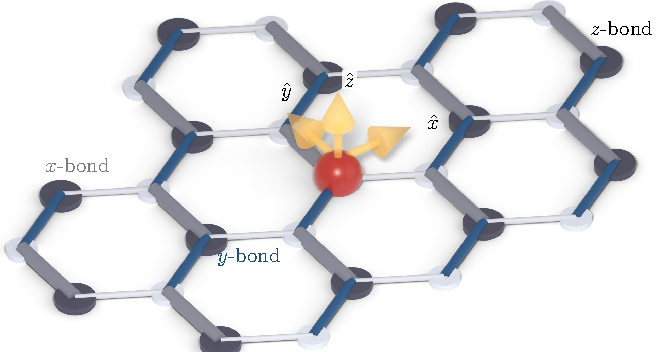
\includegraphics{figures/pdf/s06f04_kitaev.pdf}
\end{aqmfigure}


\begin{notebookbox}{\texttt{session6.ipynb}, ``(Exercise) Non-collinear magnetism from spin-orbit coupling''}
Add a Dzyaloshinskii-Moriya-type term to the mean-field Hamiltonian and watch the ground state
tilt away from collinear order, the electronic counterpart of the spin-model statement above.
\end{notebookbox}

\section{Magnons: fluctuations of the order parameter}

Up to this point we have only asked about ground states. Let us now ask about excitations. Take the
Heisenberg model (6.5) with $J<0$ (ferromagnetic), promote the spins to genuine quantum-mechanical
operators obeying the angular-momentum algebra $[S_i^a,S_j^b] = i\hbar\,\delta_{ij}\epsilon^{abc}S_i^c$
(we set $\hbar=1$ from here on, standard for this kind of calculation), and ask for its low-lying
excited states. Unlike the interacting electron problem, the ferromagnetic Heisenberg model's exact
ground state is known immediately: it is the fully polarized state, every spin aligned, since no
other configuration can lower $\langle \mathbf S_i\cdot\mathbf S_j\rangle$ any further for $J<0$. A
\textbf{magnon} is a small, propagating fluctuation of the magnetization away from this fully polarized
state: qualitatively, a single spin tipped slightly out of alignment, delocalized coherently over the
whole lattice as a wave. The question is how to extract these excitations systematically from a
genuinely many-body spin Hamiltonian, and the answer is a change of variables that turns the spin
problem into a bosonic tight-binding problem.

\section{The Holstein-Primakoff transformation}

The \textbf{Holstein-Primakoff transformation} maps spin operators exactly onto bosonic creation and
annihilation operators $a_i^\dagger, a_i$ with $[a_i,a_j^\dagger]=\delta_{ij}$. For a spin of
magnitude $S$ on site $i$,

\begin{equation}
S_i^z = S - a_i^\dagger a_i, \qquad S_i^+ = \sqrt{2S-a_i^\dagger a_i}\;a_i, \qquad S_i^- = a_i^\dagger\sqrt{2S-a_i^\dagger a_i}.
\end{equation}

This is an \emph{exact} rewriting: substituting (6.6) into the bosonic commutation relations reproduces
the full $SU(2)$ spin algebra $[S_i^z,S_i^\pm]=\pm S_i^\pm$, $[S_i^+,S_i^-]=2S_i^z$ exactly, with no
approximation yet made. The physical picture behind it is direct: $a_i^\dagger a_i$ counts how many
units of spin have been removed from the fully polarized value $S$ on site $i$, i.e. it counts
\textbf{magnons} on that site, and $S_i^z=S-a_i^\dagger a_i$ says exactly that. The square-root operator
factors are what make (6.6) exact even far from full polarization; they are also what makes the
Hamiltonian, written this way, look more complicated rather than less.

The simplification comes from linearizing: whenever the expectation value of $a_i^\dagger a_i$ stays
much smaller than $S$, i.e. whenever we stay close to the fully polarized ground state (precisely the
regime we want, since we are looking for low-lying excitations above that ground state), we can
expand the square roots and keep only the leading term,

\begin{equation}
S_i^+ \approx \sqrt{2S}\, a_i, \qquad S_i^- \approx \sqrt{2S}\, a_i^\dagger, \qquad S_i^z = S - a_i^\dagger a_i.
\end{equation}

This linearized form is the one used to compute magnon spectra in practice. The bookkeeping it
implies is worth stating plainly, since it is the cleanest way to remember the whole transformation:
$S^+$ (which \emph{raises} $S^z$, i.e. increases the local magnetization back toward saturation)
\emph{destroys} a magnon, while $S^-$ (which lowers the magnetization) \emph{creates} one; the total
magnetization of the system is the fully saturated value minus the total magnon number,
$\sum_i \langle S_i^z\rangle = NS - \sum_i\langle a_i^\dagger a_i\rangle$. Each individual magnon
carries exactly one unit of spin, so magnons are $S=1$ excitations, consistent with what we said about
them back in Section 6.1, and they exist only because the ground state they live on top of has
already spontaneously broken spin-rotation symmetry. Figure~\ref{fig:s06:magnon} draws all three
pieces: the fully polarized ground state, the delocalized precession wave that carries a single
magnon, and this raising/lowering dictionary.

% Session 6 -- what a magnon is in real space, and the Holstein-Primakoff bookkeeping.
% Placement: sec. "The Holstein-Primakoff transformation", at the paragraph that states the
% bookkeeping (S^- creates a magnon, S^+ destroys one) after eq. (6.7).
% Rendered by figures/blender/s06f05_magnon.py, labels in figures/overlays/s06f05_magnon.tex.
\begin{aqmfigure}{fig:s06:magnon}{The states that (6.6) and (6.7) describe. (a) The ferromagnetic
ground state, where every spin has its maximal value $S^z=S$, and so there are no magnons. (b) A
single magnon is \emph{not} one spin flipped on one site. Instead, every spin is tilted slightly out
of alignment and precesses on its cone, and the precession phase advances by $\mathbf
k\cdot\boldsymbol\delta$ from one site to the next. This is seen most clearly in the view from
above, where the transverse component turns at a constant rate and comes back to itself after one
wavelength. The missing unit of spin is therefore shared coherently by the whole lattice, and
$\sum_i\langle S_i^z\rangle=NS-1$. Since the tilting angle is small, we have $\langle a_i^\dagger
a_i\rangle\ll S$ everywhere, which is the condition under which we can expand the square roots in
(6.6). In the drawing the tilting angle is much larger than in reality. (c) The counting rule that
makes the transformation easy to remember. The boson number counts the spin removed from saturation,
so the \emph{lowering} operator $S^-$ creates a magnon and the \emph{raising} operator $S^+$
destroys one.}
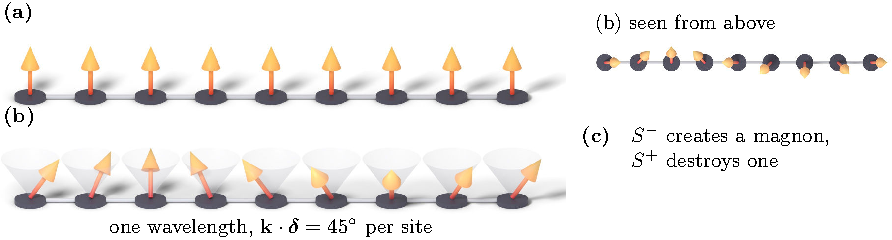
\includegraphics{figures/pdf/s06f05_magnon.pdf}
\end{aqmfigure}


Substituting (6.7) into the ferromagnetic Heisenberg Hamiltonian, $H = J\sum_{\langle ij\rangle}
\mathbf S_i\cdot\mathbf S_j = J\sum_{\langle ij\rangle}\big[S_i^zS_j^z + \tfrac12(S_i^+S_j^-+S_i^-S_j^+)\big]$,
and keeping terms up to quadratic order in the bosonic operators,

\begin{equation*}
S_i^zS_j^z \approx S^2 - S\big(a_i^\dagger a_i + a_j^\dagger a_j\big), \qquad
\tfrac12\big(S_i^+S_j^- + S_i^-S_j^+\big) \approx S\big(a_i^\dagger a_j + a_j^\dagger a_i\big),
\end{equation*}

converts the spin Hamiltonian into a bosonic tight-binding Hamiltonian for magnons, whose hopping
amplitude is set directly by the exchange coupling $J$, exactly as advertised: the magnon ``hops''
between sites with amplitude proportional to $JS$, in precise analogy with the electronic
tight-binding Hamiltonians we have diagonalized all course.

\section{Magnon dispersions: ferromagnets versus antiferromagnets}

Fourier transforming the bosonic Hamiltonian from Section 6.14 on a Bravais lattice with coordination
number $z$ and nearest-neighbor structure factor $\gamma(\mathbf k) = \tfrac1z\sum_{\boldsymbol\delta}
e^{i\mathbf k\cdot\boldsymbol\delta}$ gives, for the \textbf{ferromagnet} ($J<0$, writing $|J|=-J$), a
diagonal magnon Hamiltonian with dispersion

\begin{equation}
E_\text{FM}(\mathbf k) = |J|\,S\,z\big(1-\gamma(\mathbf k)\big).
\end{equation}

This vanishes at $\mathbf k=0$, as it must (a uniform rotation of every spin costs no energy at all,
the Goldstone mode of the broken spin-rotation symmetry), and expanding $\gamma(\mathbf k)$ for small
$\mathbf k$ gives $E_\text{FM}(\mathbf k)\propto k^2$: a \textbf{quadratic} magnon dispersion, exactly the
``gapless, quadratic'' ferromagnetic magnon the lecture flags.

The \textbf{antiferromagnetic} case needs one more step, because the ground state is not simply ``all
spins up.'' On a bipartite lattice, apply the Holstein-Primakoff transformation (6.7) separately on the
two sublattices, with the roles of $S^+$ and $S^-$ swapped on the $B$ sublattice (since those spins
point the opposite way): $S_i^z=S-a_i^\dagger a_i$ on $A$, but $S_j^z=-S+b_j^\dagger b_j$ on $B$.
Substituting into $\mathbf S_i\cdot\mathbf S_j$ for a bond between the two sublattices now produces
not just density terms $a^\dagger a$, $b^\dagger b$, but also \emph{anomalous}, particle-number-non-conserving
terms $a_i b_j$ and $a_i^\dagger b_j^\dagger$: a signature that the magnon vacuum on top of the Néel
state is not simply the bosonic vacuum, and that diagonalizing the Hamiltonian requires a Bogoliubov
transformation rather than a plain Fourier transform. Carrying that out gives the antiferromagnetic
magnon dispersion

\begin{equation}
E_\text{AFM}(\mathbf k) = J\,S\,z\,\sqrt{1-\gamma(\mathbf k)^2}.
\end{equation}

Near $\mathbf k=0$, $1-\gamma(\mathbf k)^2 \propto k^2$, so $E_\text{AFM}(\mathbf k)\propto |k|$: a
\textbf{linear}, Dirac-cone-like dispersion, gapless at the same point but linear rather than quadratic.
This is exactly the ``quadratic in ferromagnets, linear in antiferromagnets'' rule of thumb from the
lecture, now derived rather than merely quoted; it is also, incidentally, one more example (alongside
the Dirac cones of session 2 and 3) of a linear dispersion arising from the structure of a symmetry
rather than being put in by hand. Figure~\ref{fig:s06:dispersion} plots (6.8) and (6.9) together,
with the zone centre magnified so the parabola and the cone can be told apart.

% Session 6 -- ferromagnetic versus antiferromagnetic magnon dispersions, eqs. (6.8) and (6.9).
% Placement: sec. "Magnon dispersions: ferromagnets versus antiferromagnets", after eq. (6.9)
% and the "quadratic in ferromagnets, linear in antiferromagnets" paragraph.
% Rendered by figures/blender/s06f06_dispersion.py, labels in figures/overlays/s06f06_dispersion.tex.
\begin{aqmfigure}{fig:s06:dispersion}{Magnon dispersions (6.8) and (6.9) for a chain ($z=2$,
$\gamma(\mathbf k)=\cos ka$), both in units of $|J|Sz$. Both are zero at $\mathbf k=0$, since a
uniform rotation of all the spins costs no energy. So the magnon is the Goldstone mode of the broken
spin-rotation symmetry, and no value of the exchange can open a gap in it. The difference is
\emph{how} the two dispersions go to zero. The factor $1-\gamma(\mathbf k)$ of the ferromagnet is
quadratic in $k$. The factor $\sqrt{1-\gamma(\mathbf k)^2}$ of the antiferromagnet is the square
root of the same quantity, so it is linear and gives a Dirac-like cone instead of a parabola. The
right panel magnifies the zone centre, where the difference is clear. This extra square root comes
from the Bogoliubov transformation that the N\'eel state requires, since the anomalous $a_ib_j$
terms are what change a parabola into a cone.}
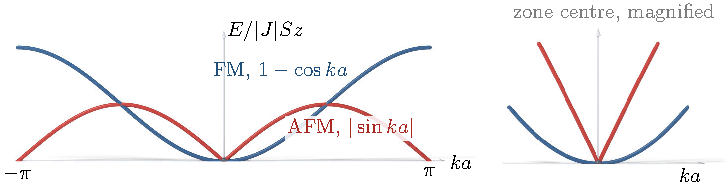
\includegraphics{figures/pdf/s06f06_dispersion.pdf}
\end{aqmfigure}


\section{Topological magnons}

Once magnons have a genuine band structure, a dispersion $E(\mathbf k)$ over the Brillouin zone, the
same question we have already asked twice about \emph{electronic} bands becomes available to ask about
\emph{magnon} bands: can that band structure carry a nontrivial topological invariant? This is precisely
the Chern-number machinery from sessions 3 and 4 (Berry curvature $\Omega(\mathbf k)$ of a Bloch band,
integrated over the Brillouin zone to give an integer,

\begin{equation}
C = \frac{1}{2\pi}\int_\text{BZ} \Omega(\mathbf k)\, d^2k,
\end{equation}

applied a third time, now to the bosonic Bogoliubov Hamiltonian of Section 6.15 instead of an
electronic tight-binding Hamiltonian. Adding spin-orbit coupling on top of the plain Heisenberg
exchange, of the Dzyaloshinskii-Moriya type from Section 6.12, plays exactly the role that the
Haldane model's complex second-neighbor hopping played for electrons back in session 4: it introduces
complex phases into the magnon hopping amplitudes, which can open a gap in the magnon band structure
at finite energy and endow the bands on either side of that gap with a nonzero Chern number (6.10).
When such a topological magnon Hamiltonian is put on a ribbon geometry, bulk-boundary correspondence
guarantees chiral magnon edge modes living in the gap, propagating in one direction only along each
edge, the magnon analogue of the chiral electronic edge states of a Chern insulator. These modes carry
spin and energy, not charge, but they are topologically protected in exactly the same sense as their
electronic counterparts: the same tool we used for electrons in sessions 3 and 4, now applied to
magnon bands.

\begin{notebookbox}{\texttt{session6.ipynb}, ``(Exercise) Topological magnons in 2D magnets''}
Build a magnon Hamiltonian with a Dzyaloshinskii-Moriya-type spin-orbit term on top of Heisenberg
exchange, compute its Chern number via (6.10), and check for chiral edge magnon modes on a ribbon,
directly reproducing the bulk-boundary correspondence argument above in the magnon setting.
\end{notebookbox}

A brief note on scope before we stop: the companion notebook goes further than this session's lecture
in a few places, most visibly its exercises on electronic and magnetic symmetry breaking in graphene
multilayers, and its closing sections on many-body spin response functions. Those are genuine,
worthwhile extensions of today's material, but since neither the transcript nor the slides for this
session narrate them, we have not built the corresponding derivations into these notes; treat them as
independent notebook exploration rather than as material these notes derive.

\section{Closing summary}

So far in this session we have:

\begin{itemize}
\item Rebuilt Hubbard-model magnetism numerically in full depth, including the direct competition
  between ferromagnetic and antiferromagnetic self-consistent solutions and the Stoner threshold
  (6.3) that decides whether magnetism appears at all.
\item Derived the Heisenberg model rigorously from the strongly correlated Hubbard limit, getting the
  exact coefficient $J=4t^2/U$ (6.4) and its lattice generalization (6.5), including how frustration
  and superexchange modify that simple picture.
\item Built the magnon spectrum from first principles via the Holstein-Primakoff transformation
  (6.6)--(6.7), getting the quadratic ferromagnetic dispersion (6.8) and linear antiferromagnetic
  dispersion (6.9), and then extended session 3 and 4's topological machinery a third time to show
  that magnon bands can be topological too.
\end{itemize}

And that is exactly where the live lecture leaves us: right after topological magnons, with no
narrated take-home slide. This is a genuine feature of this year's recording, not a gap in these
notes, so we end here too rather than inventing a summary sentence the lecture never says. Every
magnet we have built today, from the mean-field exchange field all the way to the topological magnon
edge states, is a state that breaks time-reversal symmetry: some net, staggered, or noncollinear spin
arrangement that looks different run backwards in time from how it looks run forwards.

Two threads are left dangling on purpose, both flagged along the way rather than resolved here. The
Kitaev interaction of Section 6.12, singled out explicitly as ``important for quantum spin liquids,''
is picked up from two different directions in the sessions ahead: session 7 treats the
frustrated, kagome-type Hamiltonians it belongs to as the paradigm case where mean-field theory
simply fails, while session 8 returns to the Kitaev model itself as a route to an exactly solvable
quantum spin liquid. And the spinon, previewed only by name and by its spin-$1/2$, charge-neutral
quantum numbers back in Section 6.1, gets the same full treatment magnons received today, only in
session 8, once we turn from magnets that break time-reversal symmetry to quantum magnets that do
not.
